\documentclass[16pt]{article}
%\usepackage{caption}
\usepackage{setspace,graphicx,epstopdf,amsmath,amsfonts,amssymb,amsthm}
\usepackage{marginnote,datetime,enumitem,subfigure,rotating,fancyvrb}
\usepackage{hyperref,float}
\usepackage[longnamesfirst]{natbib}
\usepackage{mathtools}
\usepackage{caption}
\usepackage{float}
\usepackage{lscape}
\usepackage{graphicx}
\usepackage{flafter} 
\usepackage{tabularx} 
\usepackage{booktabs}
\usepackage{changepage}
\usepackage{setspace}
\usepackage{placeins}
\usepackage{threeparttable}
\usepackage{ragged2e}
\usepackage[export]{adjustbox}
\newcolumntype{Y}{>{\raggedleft\arraybackslash}X}% raggedleft column X
\usdate
\usepackage[a4paper,bindingoffset=0.2in,%
            left=1.1in,right=0.85in,top=1in,bottom=1in,%
            footskip=.25in]{geometry}

\begin{document}

% this stuff is about to be presented to Alan on 09/(02-04)/19

% the scripts used:
% sp19_rm_22 for all monthly tables
% sp19_dailycimad_betas_7_49 for Figure 1.
% sp19_annually, semiannualy, quarterly_2.
% sp19_rm_21_5-10-17-30-49 for industries tables
% sp19_industry_partitions for short industry tables.

\newgeometry{left=1.5cm, right=1cm, top=3cm, bottom=1.5cm}




\newpage


\section{Introduction} \label{sec:Model}

\section{Data and Dispersion Measures} \label{sec:Model}
\subsection{Sample}
\subsection{Construction of Dispersion Measures}


\section{Asset Pricing Results} \label{sec:Model}
\subsection{Estimation of $\beta_{CID}$}
\subsection{Portfolios, formed on $\beta_{CID}$}
\subsection{Cross-sectional Results}
\subsection{Performance of different Dispersion Measures}


\section{Economic Channel: Labor Income Risk} \label{sec:Model}
\subsection{Economic Mechanism and Hypotheses}
\subsection{Results}


\section{Further results} \label{sec:Model}
\subsection{Robustness to different industry definitions}
\subsection{Robustness to other uncertainty measures}
\subsection{Results at lower frequency}
\subsection{Economic and financial forecasting power of CIV}

\section{Conclusion} \label{sec:Model}



\newpage

\newgeometry{left=2.5cm, right=0.75cm, top=1.75cm, bottom=1.5cm}

\begin{figure*}
\textbf{Figure 1: Dispersion Measures}
\vskip 6 pt
\begin{flushleft}
{The plot describes time series of cross-sectional dispersion (CSD), cross-industry dispersion (CID) and within-industry dispersion (WID). All the measures are calculated as mean absolute deviation of the returns at daily frequency. Industries are defined according to Fama-French 49 industry classification. The paper uses value-weighted industry returns to calculate CID.}
\end{flushleft}
\centering
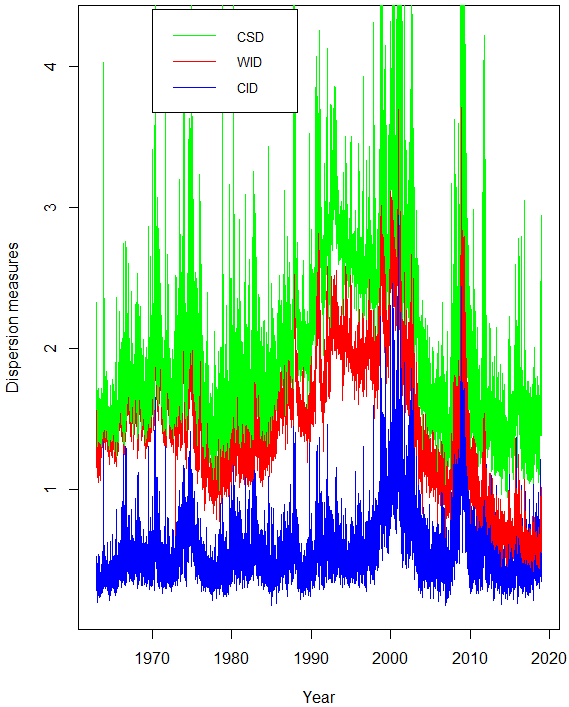
\includegraphics[width=1\textwidth]{fig1.png}
\end{figure*}


\begin{figure*}
\textbf{Figure 2: Postranking $\beta_{CID}$}
\vskip 12 pt
\begin{flushleft}
{The plot describes the relationship between postranking and preranking $\beta_{CID}$ of decile portfolios, sorted on $\beta_{CID}$.}
\end{flushleft}
\centering
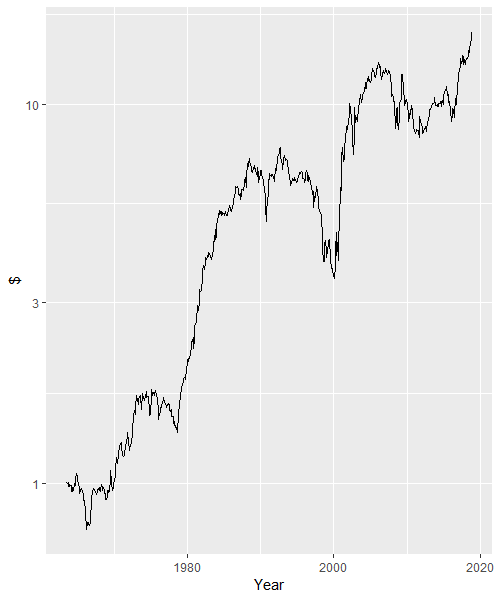
\includegraphics[width=1\textwidth]{Figure2.png}
\end{figure*}


\begin{figure*}
\textbf{Figure 3: Performance of \$1 (log scale)}
\vskip 12 pt
\begin{flushleft}
{The plot describes growth of the investment of \$1 in one of the three portfolios. L/S5 (L/S10) corresponds to long-short portfolio, defined as a difference in returns of extreme quintile (decile) portfolios. Mkt is the value-weighted return of all CRSP stocks(vwretd).}
\end{flushleft}
\centering
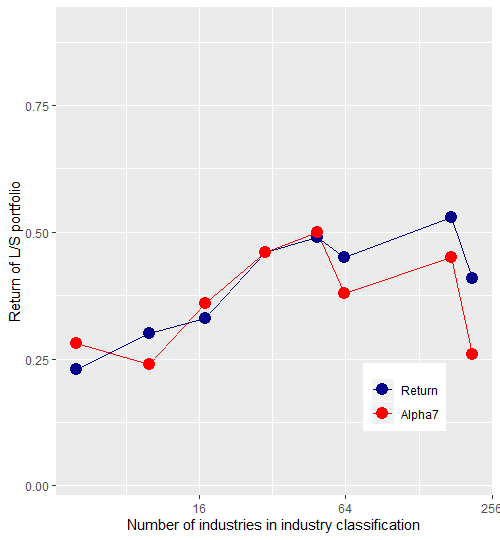
\includegraphics[width=1\textwidth]{Figure3.png}
\end{figure*}


\begin{figure*}
\textbf{Figure 4: Returns of decile L/S portfolio using different Fama-French industry partitions}
\vskip 12 pt
\begin{flushleft}
{The plot describes monthly returns and abnormal returns of decile L/S portfolios, formed on $\beta_{CID}$. I use Fama-French industry definitions with different coarseness: 49, 30, 17, 10 and 5 industries to compute CID. Abnormal returns are calculated with respect to Fama-French 5 factor model, including Momentum and Short-term Reversal factors.}
\end{flushleft}
\centering
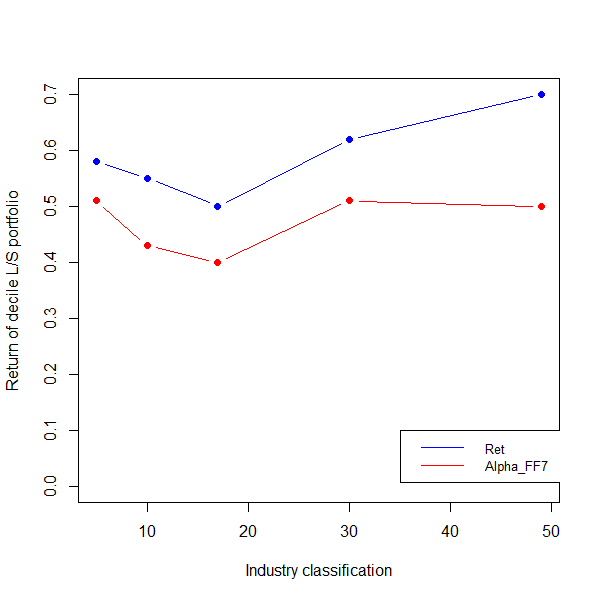
\includegraphics[width=1\textwidth]{alphas_inds.png}
\end{figure*}


\clearpage


% Table created by stargazer v.5.2.2 by Marek Hlavac, Harvard University. E-mail: hlavac at fas.harvard.edu
% Date and time: Tue, Sep 03, 2019 - 1:38:31 PM
\begin{table}[!htbp] \centering 
  \caption{Correlations of changes in CID with changes of other variables} 
  \label{} 
    \begin{flushleft}
    {\medskip\small
 The table reports correlations between changes in CID and changes in other variables at monthly frequency. VIX is implied volatility, available starting from 1990. FU and MU are financial and macroeconomic uncertainty from Sydney Ludvigson website. VOL is the volatility of monthly value-weighted market index over recent 24 months. CIV is common idosyncratic volatility (Kelly et al., 2016). }
    \medskip
    \end{flushleft}
\begin{tabular}{@{\extracolsep{5pt}} ccccccc} 
\\[-1.8ex]\hline 
\hline \\[-1.8ex] 
 & VIX & FU & MU & VOL & CIV & CID \\ 
\hline \\[-1.8ex] 
VIX & $1$ & $0.40$ & $0.36$ & $0.34$ & $0.50$ & $0.12$ \\ 
FU & $0.40$ & $1$ & $0.44$ & $0.30$ & $0.39$ & $0.26$ \\ 
MU & $0.36$ & $0.44$ & $1$ & $0.11$ & $0.24$ & $0.09$ \\ 
VOL & $0.34$ & $0.30$ & $0.11$ & $1$ & $0.27$ & $0.29$ \\ 
CIV & $0.50$ & $0.39$ & $0.24$ & $0.27$ & $1$ & $0.30$ \\ 
CID & $0.12$ & $0.26$ & $0.09$ & $0.29$ & $0.30$ & $1$ \\ 
\hline \\[-1.8ex] 
\end{tabular} 
\end{table}


\textbf{Results with monthly returns:}


% Table created by stargazer v.5.2.2 by Marek Hlavac, Harvard University. E-mail: hlavac at fas.harvard.edu
% Date and time: Tue, Sep 03, 2019 - 1:39:07 PM
\begin{table}[!htbp] \centering 
  \caption{Characteristics of decile $\beta_{CID}$-sorted vw portfolios} 
  \label{} 
      \begin{flushleft}
    {\medskip\small
 The table reports mean values of characteristics of decile portfolios, sorted on $\beta_{CID}$. Size is log of market equity in the previous month. bm is log of Book-to-Market. op is operating profitability. BAspr is average bid-ask spread as a percentage of average price over the previous month. }
    \medskip
    \end{flushleft}
\begin{tabular}{@{\extracolsep{0pt}} lccccccccccc} 
\\[-1.8ex]\hline 
\hline \\[-1.8ex] 
 & D1 & D2 & D3 & D4 & D5 & D6 & D7 & D8 & D9 & D10 & LS \\ 
\hline \\[-1.8ex] 
RET & $1.17$ & $0.88$ & $0.86$ & $0.71$ & $0.63$ & $0.65$ & $0.65$ & $0.60$ & $0.52$ & $0.47$ & $$-$0.70$ \\ 
RET\_tstat & $4.80$ & $4.38$ & $4.56$ & $3.97$ & $3.73$ & $3.87$ & $3.69$ & $3.48$ & $2.79$ & $2.12$ & $$-$3.87$ \\ 
preranking beta & $$-$1.55$ & $$-$0.86$ & $$-$0.51$ & $$-$0.26$ & $$-$0.05$ & $0.16$ & $0.38$ & $0.62$ & $0.96$ & $1.62$ & $3.16$ \\ 
postranking beta & $$-$0.03$ & $0.12$ & $0.18$ & $0.23$ & $0.31$ & $0.32$ & $0.33$ & $0.41$ & $0.46$ & $0.58$ & $0.62$ \\ 
size & $7.11$ & $7.71$ & $8.13$ & $8.37$ & $8.60$ & $8.81$ & $8.96$ & $9.16$ & $9.15$ & $8.85$ & $1.74$ \\ 
bm & $6.05$ & $6.12$ & $6.13$ & $6.14$ & $6.14$ & $6.11$ & $6.11$ & $6.07$ & $6.01$ & $5.97$ & $$-$0.08$ \\ 
op & $0.15$ & $0.16$ & $0.17$ & $0.17$ & $0.17$ & $0.17$ & $0.17$ & $0.18$ & $0.18$ & $0.17$ & $0.02$ \\ 
inv & $0.29$ & $0.23$ & $0.18$ & $0.16$ & $0.14$ & $0.13$ & $0.13$ & $0.14$ & $0.14$ & $0.17$ & $$-$0.12$ \\ 
beta & $1.07$ & $0.96$ & $0.91$ & $0.88$ & $0.88$ & $0.89$ & $0.92$ & $0.98$ & $1.08$ & $1.31$ & $0.23$ \\ 
BAspr & $0.39$ & $0.32$ & $0.26$ & $0.24$ & $0.23$ & $0.21$ & $0.20$ & $0.19$ & $0.18$ & $0.18$ & $$-$0.21$ \\ 
mom122 & $0.24$ & $0.18$ & $0.15$ & $0.14$ & $0.12$ & $0.12$ & $0.11$ & $0.11$ & $0.11$ & $0.14$ & $$-$0.10$ \\ 
vol1m & $2.47$ & $2.02$ & $1.82$ & $1.72$ & $1.66$ & $1.61$ & $1.60$ & $1.63$ & $1.74$ & $2.03$ & $$-$0.44$ \\ 
vol12m & $2.63$ & $2.12$ & $1.90$ & $1.79$ & $1.72$ & $1.68$ & $1.67$ & $1.71$ & $1.83$ & $2.19$ & $$-$0.43$ \\ 
\hline \\[-1.8ex] 
\end{tabular} 
\end{table}




% Table created by stargazer v.5.2.2 by Marek Hlavac, Harvard University. E-mail: hlavac at fas.harvard.edu
% Date and time: Tue, Sep 03, 2019 - 2:31:38 PM
\begin{table}[!htbp] \centering 
  \caption{Returns of decile $\beta_{CID}$-sorted portfolios} 
  \label{} 
\begin{tabular}{@{\extracolsep{-5pt}} cccccccccccc} 
\\[-1.8ex]\hline 
\hline \\[-1.8ex] 
 & D1 & D2 & D3 & D4 & D5 & D6 & D7 & D8 & D9 & D10 & LS \\ 
\hline \\[-1.8ex] 
Mean ew & 2.50 & 1.79$^{***}$ & 1.58$^{***}$ & 1.41$^{***}$ & 1.36$^{***}$ & 1.32$^{***}$ & 1.29$^{***}$ & 1.26$^{***}$ & 1.29$^{***}$ & 1.61$^{***}$ & -0.89$^{***}$ \\ 
T-stat ew & 9.65 & 8.70 & 8.15 & 7.73 & 7.48 & 7.26 & 6.84 & 6.52 & 6.34 & 6.45 & -5.72 \\ 
Mean vw & 1.17 & 0.88$^{***}$ & 0.86$^{***}$ & 0.71$^{***}$ & 0.63$^{***}$ & 0.65$^{***}$ & 0.65$^{***}$ & 0.60$^{***}$ & 0.52$^{***}$ & 0.47$^{**}$ & -0.70$^{***}$ \\ 
T-stat vw & 4.80 & 4.38 & 4.56 & 3.97 & 3.73 & 3.87 & 3.69 & 3.48 & 2.79 & 2.12 & -3.87 \\ 
\hline \\[-1.8ex] 
\end{tabular} 
\end{table}



% Table created by stargazer v.5.2.2 by Marek Hlavac, Harvard University. E-mail: hlavac at fas.harvard.edu
% Date and time: Tue, Sep 03, 2019 - 1:44:52 PM
\begin{table}[!htbp] \centering 
  \caption{Abnormal returns of decile $\beta_{CID}$-sorted vw portfolios} 
  \label{} 
\begin{tabular}{@{\extracolsep{0pt}} ccccccc} 
\\[-1.8ex]\hline 
\hline \\[-1.8ex] 
Statistic & Ret & $\alpha_{CAPM}$ & $\alpha_{FF3}$ & $\alpha_{Carhart}$ & $\alpha_{FF5}$ & $\alpha_{FF5+UMD+STR}$ \\ 
\hline \\[-1.8ex] 
LS & -0.70$^{***}$ & -0.67$^{***}$ & -0.75$^{***}$ & -0.55$^{***}$ & -0.80$^{***}$ & -0.50$^{***}$ \\ 
 & [ -3.87] & [ -3.68] & [ -4.44] & [ -3.24] & [ -4.59] & [ -2.90] \\ 
\hline \\[-1.8ex] 
\end{tabular} 
\end{table}



% Table created by stargazer v.5.2.2 by Marek Hlavac, Harvard University. E-mail: hlavac at fas.harvard.edu
% Date and time: Tue, Sep 03, 2019 - 1:45:59 PM
\begin{table}[!htbp] \centering 
  \caption{Factor loadings of decile $\beta_{CID}$-sorted vw portfolios} 
  \label{} 
\begin{tabular}{@{\extracolsep{0pt}} ccccccccccc} 
\\[-1.8ex]\hline 
\hline \\[-1.8ex] 
Decile & Ret & Alpha & EMKT & HML & SMB & RMW & CMA & Mom & STR & adjR2 \\ 
\hline \\[-1.8ex] 
1 & 1.17 & 0.57 & 1.03 & -0.07 & 0.42 & -0.23 & -0.34 & 0.16 & 0.12 & 0.83 \\ 
 & [ 4.80] & [ 5.24] & [ 38.82] & [ -1.37] & [ 11.75] & [ -4.61] & [ -4.57] & [ 6.39] & [ 3.41] &  \\ 
2 & 0.88 & 0.22 & 0.97 & 0.05 & 0.23 & 0.07 & -0.15 & 0.12 & 0.10 & 0.84 \\ 
 & [ 4.38] & [ 2.46] & [ 45.09] & [ 1.18] & [ 7.84] & [ 1.63] & [ -2.43] & [ 5.67] & [ 3.48] &  \\ 
3 & 0.86 & 0.28 & 0.95 & 0.03 & 0.13 & -0.02 & -0.10 & 0.12 & 0.04 & 0.84 \\ 
 & [ 4.56] & [ 3.40] & [ 47.65] & [ 0.66] & [ 4.98] & [ -0.45] & [ -1.75] & [ 6.48] & [ 1.60] &  \\ 
4 & 0.71 & 0.07 & 0.96 & 0.03 & 0.08 & 0.14 & 0.05 & 0.08 & 0.07 & 0.86 \\ 
 & [ 3.97] & [ 0.92] & [ 54.98] & [ 1.00] & [ 3.56] & [ 4.13] & [ 1.03] & [ 4.67] & [ 2.99] &  \\ 
5 & 0.63 & 0.00 & 0.94 & 0.04 & 0.08 & 0.14 & 0.17 & 0.05 & 0.01 & 0.88 \\ 
 & [ 3.73] & [ -0.02] & [ 60.62] & [ 1.43] & [ 3.60] & [ 4.91] & [ 3.97] & [ 3.37] & [ 0.64] &  \\ 
6 & 0.65 & 0.07 & 0.92 & 0.02 & -0.01 & 0.13 & 0.10 & 0.02 & 0.06 & 0.88 \\ 
 & [ 3.87] & [ 1.20] & [ 60.34] & [ 0.70] & [ -0.27] & [ 4.62] & [ 2.33] & [ 1.38] & [ 3.11] &  \\ 
7 & 0.65 & 0.08 & 0.98 & 0.03 & -0.04 & 0.11 & 0.13 & -0.02 & 0.05 & 0.90 \\ 
 & [ 3.69] & [ 1.36] & [ 67.63] & [ 1.10] & [ -1.81] & [ 3.84] & [ 3.25] & [ -1.65] & [ 2.72] &  \\ 
8 & 0.60 & 0.03 & 1.01 & 0.12 & -0.08 & 0.18 & 0.12 & -0.04 & 0.00 & 0.91 \\ 
 & [ 3.48] & [ 0.47] & [ 74.54] & [ 4.69] & [ -4.30] & [ 7.16] & [ 3.14] & [ -2.98] & [ -0.24] &  \\ 
9 & 0.52 & 0.04 & 1.03 & 0.07 & -0.10 & 0.05 & 0.08 & -0.09 & -0.03 & 0.88 \\ 
 & [ 2.79] & [ 0.60] & [ 60.97] & [ 2.13] & [ -4.17] & [ 1.59] & [ 1.59] & [ -5.27] & [ -1.37] &  \\ 
10 & 0.47 & 0.07 & 1.16 & 0.14 & -0.04 & -0.12 & -0.11 & -0.13 & -0.13 & 0.83 \\ 
 & [ 2.12] & [ 0.71] & [ 47.98] & [ 3.07] & [ -1.15] & [ -2.71] & [ -1.64] & [ -5.54] & [ -3.96] &  \\ 
LS & -0.70 & -0.50 & 0.13 & 0.21 & -0.46 & 0.11 & 0.23 & -0.29 & -0.25 & 0.23 \\ 
 & [ -3.87] & [ -2.90] & [ 3.04] & [ 2.62] & [ -8.05] & [ 1.35] & [ 1.94] & [ -7.20] & [ -4.41] &  \\ 
\hline \\[-1.8ex] 
\end{tabular} 
\end{table} 



% Table created by stargazer v.5.2.2 by Marek Hlavac, Harvard University. E-mail: hlavac at fas.harvard.edu
% Date and time: Tue, Sep 03, 2019 - 1:47:00 PM
\begin{table}[!htbp] \centering 
  \caption{Abnormal returns of 2x3 doublesorted portfolios on size and $\beta_{CID}$} 
  \label{} 
\begin{tabular}{@{\extracolsep{5pt}} ccccccc} 
\\[-1.8ex]\hline 
\hline \\[-1.8ex] 
Statistic & Ret & $\alpha_{CAPM}$ & $\alpha_{FF3}$ & $\alpha_{Carhart}$ & $\alpha_{FF5}$ & $\alpha_{FF5+UMD+STR}$ \\ 
\hline \\[-1.8ex] 
L/S Size & 0.74$^{***}$ & 0.67$^{***}$ & 0.51$^{***}$ & 0.56$^{***}$ & 0.47$^{***}$ & 0.52$^{***}$ \\ 
T-stat & [ 7.38] & [ 6.84] & [ 12.35] & [ 13.92] & [ 11.30] & [ 12.66] \\ 
L/S CID & 0.22$^{**}$ & 0.23$^{**}$ & 0.28$^{***}$ & 0.15 & 0.31$^{***}$ & 0.16 \\ 
T-stat & [ 2.24] & [ 2.40] & [ 2.91] & [ 1.59] & [ 3.13] & [ 1.61] \\ 
\hline \\[-1.8ex] 
\end{tabular} 
\end{table}



% Table created by stargazer v.5.2.2 by Marek Hlavac, Harvard University. E-mail: hlavac at fas.harvard.edu
% Date and time: Wed, Sep 04, 2019 - 10:02:03 AM
\begin{table}[!htbp] \centering 
  \caption{Fama-MacBeth regression} 
  \label{} 
\begin{tabular}{@{\extracolsep{0pt}}lccccccc} 
\\[-1.8ex]\hline 
\hline \\[-1.8ex] 
 & \multicolumn{7}{c}{\textit{Dependent variable: Return}} \\ 
\cline{2-8} 
\\[-1.8ex] & (1) & (2) & (3) & (4) & (5) & (6) & (7)\\ 
\hline \\[-1.8ex] 
 $\beta_{CID}$ & $-$0.30$^{***}$ & $-$0.31$^{***}$ & $-$0.09$^{**}$ & $-$0.10$^{**}$ & $-$0.09$^{**}$ & $-$0.09$^{***}$ & $-$0.09$^{***}$ \\ 
  & [ $-$4.64] & [ $-$6.50] & [ $-$2.45] & [ $-$2.53] & [ $-$2.39] & [ $-$2.60] & [ $-$2.60] \\ 
  & & & & & & & \\ 
 $\beta_{MKT}$ &  & 0.31 & 0.69$^{***}$ & 0.71$^{***}$ & 0.64$^{***}$ & 0.72$^{***}$ & 0.62$^{***}$ \\ 
  &  & [ 1.54] & [ 3.11] & [ 3.35] & [ 3.17] & [ 3.59] & [ 3.25] \\ 
  & & & & & & & \\ 
 size &  &  & $-$0.63$^{***}$ & $-$0.62$^{***}$ & $-$0.62$^{***}$ & $-$0.62$^{***}$ & $-$0.58$^{***}$ \\ 
  &  &  & [ $-$14.36] & [ $-$13.63] & [ $-$13.98] & [ $-$14.24] & [ $-$14.57] \\ 
  & & & & & & & \\ 
 logbm &  &  &  & 0.04 & 0.05 & $-$0.02 & 0.004 \\ 
  &  &  &  & [ 0.77] & [ 0.90] & [ $-$0.28] & [ 0.07] \\ 
  & & & & & & & \\ 
 mom122 &  &  &  &  & 0.04 & 0.01 & 0.02 \\ 
  &  &  &  &  & [ 0.22] & [ 0.04] & [ 0.13] \\ 
  & & & & & & & \\ 
 inv &  &  &  &  &  & $-$1.23$^{***}$ & $-$1.25$^{***}$ \\ 
  &  &  &  &  &  & [ $-$8.34] & [ $-$8.51] \\ 
  & & & & & & & \\ 
 MAX &  &  &  &  &  &  & 0.02$^{***}$ \\ 
  &  &  &  &  &  &  & [ 3.21] \\ 
  & & & & & & & \\ 
 Constant & 1.49$^{***}$ & 1.21$^{***}$ & 4.58$^{***}$ & 4.51$^{***}$ & 4.49$^{***}$ & 4.56$^{***}$ & 4.26$^{***}$ \\ 
  & [ 7.61] & [ 9.42] & [ 16.03] & [ 15.68] & [ 15.93] & [ 16.38] & [ 16.41] \\ 
  & & & & & & & \\ 
\hline \\[-1.8ex] 
Observations & 1,254,089 & 1,254,089 & 1,254,089 & 1,254,089 & 1,253,020 & 1,226,228 & 1,226,045 \\ 
Adjusted R$^{2}$ & 0.01 & 0.04 & 0.05 & 0.06 & 0.07 & 0.07 & 0.07 \\ 
\hline 
\hline \\[-1.8ex] 
\textit{Note:}  & \multicolumn{7}{r}{$^{*}$p$<$0.1; $^{**}$p$<$0.05; $^{***}$p$<$0.01} \\ 
\end{tabular} 
\end{table}


\clearpage


% Table created by stargazer v.5.2.2 by Marek Hlavac, Harvard University. E-mail: hlavac at fas.harvard.edu
% Date and time: Tue, Sep 03, 2019 - 1:47:48 PM
\begin{table}[!htbp] \centering 
  \caption{Abnormal returns of 5x5 doublesorted portfolios on within-industry dispersion $\beta_{WID}$ and $\beta_{CID}$} 
  \label{} 
\begin{tabular}{@{\extracolsep{5pt}} ccccccc} 
\\[-1.8ex]\hline 
\hline \\[-1.8ex] 
Statistic & Ret & $\alpha_{CAPM}$ & $\alpha_{FF3}$ & $\alpha_{Carhart}$ & $\alpha_{FF5}$ & $\alpha_{FF5+UMD+STR}$ \\ 
\hline \\[-1.8ex] 
L/S WID & 0.13 & 0.22 & 0.09 & -0.03 & -0.16 & -0.19 \\ 
T-stat & [ 0.89] & [ 1.46] & [ 0.61] & [ -0.19] & [ -1.08] & [ -1.27] \\ 
L/S CID & 0.38$^{***}$ & 0.34$^{**}$ & 0.44$^{***}$ & 0.38$^{***}$ & 0.59$^{***}$ & 0.43$^{***}$ \\ 
T-stat & [ 2.75] & [ 2.33] & [ 3.16] & [ 2.72] & [ 4.27] & [ 3.06] \\ 
\hline \\[-1.8ex] 
\end{tabular} 
\end{table}



% Table created by stargazer v.5.2.2 by Marek Hlavac, Harvard University. E-mail: hlavac at fas.harvard.edu
% Date and time: Tue, Sep 03, 2019 - 1:48:32 PM
\begin{table}[!htbp] \centering 
  \caption{Abnormal returns of 5x5 doublesorted portfolios on cross-sectional dispersion $\beta_{CSD}$ and $\beta_{CID}$} 
  \label{} 
\begin{tabular}{@{\extracolsep{5pt}} ccccccc} 
\\[-1.8ex]\hline 
\hline \\[-1.8ex] 
Statistic & Ret & $\alpha_{CAPM}$ & $\alpha_{FF3}$ & $\alpha_{Carhart}$ & $\alpha_{FF5}$ & $\alpha_{FF5+UMD+STR}$ \\  
\hline \\[-1.8ex] 
L/S CSD & -0.03 & 0.07 & -0.03 & -0.15 & -0.21 & -0.32$^{**}$ \\ 
T-stat & [ -0.20] & [ 0.49] & [ -0.24] & [ -1.06] & [ -1.52] & [ -2.24] \\ 
L/S CID & 0.32$^{**}$ & 0.28$^{**}$ & 0.30$^{**}$ & 0.26$^{**}$ & 0.43$^{***}$ & 0.31$^{**}$ \\ 
T-stat & [ 2.46] & [ 2.06] & [ 2.36] & [ 2.00] & [ 3.31] & [ 2.38] \\ 
\hline \\[-1.8ex] 
\end{tabular} 
\end{table}


\clearpage


\begin{table}[!htbp] \centering 
  \caption{Abnormal returns of 5x5 doublesorted portfolios on cross-sectional dispersion $\beta_{CSD}$ and other variables} 
  \label{} 
\begin{tabularx}{\linewidth}{p{2cm}p{1.5cm}p{1.5cm}p{1.5cm}p{1.5cm}p{1.5cm}p{1.5cm}}
    \toprule
    \multicolumn{7}{l}{\textbf{Panel A: VIX vs CID}} \\
    \midrule  
\\[-1.8ex]\hline 
\hline \\[-1.8ex] 
Statistic & Ret & $\alpha_{CAPM}$ & $\alpha_{FF3}$ & $\alpha_{Carhart}$ & $\alpha_{FF5}$ & $\alpha_{FF5+UMD+STR}$ \\ 
\hline \\[-1.8ex] 
L/S VIX & 0.25 & -0.13 & -0.09 & 0.05 & 0.19 & 0.28 \\ 
T-stat & [ 1.08] & [ -0.68] & [ -0.49] & [ 0.30] & [ 1.10] & [ 1.61] \\ 
L/S CID & 0.24 & 0.24 & 0.38$^{**}$ & 0.22 & 0.30 & 0.15 \\ 
T-stat & [ 1.20] & [ 1.19] & [ 2.12] & [ 1.24] & [ 1.64] & [ 0.87] \\ 
\hline \\[-1.8ex] 
\end{tabularx} 

\begin{tabularx}{\linewidth}{p{2cm}p{1.5cm}p{1.5cm}p{1.5cm}p{1.5cm}p{1.5cm}p{1.5cm}}
    \toprule
    \multicolumn{7}{l}{\textbf{Panel B: CIV vs CID}} \\
    \midrule  
\\[-1.8ex]\hline 
\hline \\[-1.8ex] 
Statistic & Ret & $\alpha_{CAPM}$ & $\alpha_{FF3}$ & $\alpha_{Carhart}$ & $\alpha_{FF5}$ & $\alpha_{FF5+UMD+STR}$ \\ 
\hline \\[-1.8ex] 
L/S CIV & 0.33$^{***}$ & 0.27$^{**}$ & 0.16 & 0.21$^{*}$ & 0.08 & 0.13 \\ 
T-stat & [ 2.75] & [ 2.25] & [ 1.41] & [ 1.76] & [ 0.66] & [ 1.04] \\ 
L/S CID & 0.37$^{***}$ & 0.39$^{***}$ & 0.42$^{***}$ & 0.26$^{**}$ & 0.44$^{***}$ & 0.23$^{**}$ \\ 
T-stat & [ 3.06] & [ 3.22] & [ 3.64] & [ 2.27] & [ 3.70] & [ 1.99] \\ 
\hline \\[-1.8ex] 
\end{tabularx} 


\begin{tabularx}{\linewidth}{p{2cm}p{1.5cm}p{1.5cm}p{1.5cm}p{1.5cm}p{1.5cm}p{1.5cm}}
    \toprule
    \multicolumn{7}{l}{\textbf{Panel C: Macroeconomic uncertainty (Ludvigson15) vs CID}} \\
    \midrule  
\\[-1.8ex]\hline 
\hline \\[-1.8ex] 
Statistic & Ret & $\alpha_{CAPM}$ & $\alpha_{FF3}$ & $\alpha_{Carhart}$ & $\alpha_{FF5}$ & $\alpha_{FF5+UMD+STR}$ \\ 
\hline \\[-1.8ex] 
L/S MU & 0.05 & -0.07 & -0.03 & 0.08 & 0.19 & 0.19 \\ 
T-stat & [ 0.33] & [ -0.50] & [ -0.20] & [ 0.56] & [ 1.43] & [ 1.44] \\ 
L/S CID & 0.49$^{***}$ & 0.49$^{***}$ & 0.53$^{***}$ & 0.35$^{***}$ & 0.54$^{***}$ & 0.32$^{**}$ \\ 
T-stat & [ 3.76] & [ 3.74] & [ 4.19] & [ 2.82] & [ 4.20] & [ 2.55] \\ 
\hline \\[-1.8ex] 
\end{tabularx} 

\begin{tabularx}{\linewidth}{p{2cm}p{1.5cm}p{1.5cm}p{1.5cm}p{1.5cm}p{1.5cm}p{1.5cm}}
    \toprule
    \multicolumn{7}{l}{\textbf{Panel D: Financial uncertainty (Ludvigson15) vs CID}} \\
    \midrule 
\\[-1.8ex]\hline 
\hline \\[-1.8ex] 
Statistic & Ret & $\alpha_{CAPM}$ & $\alpha_{FF3}$ & $\alpha_{Carhart}$ & $\alpha_{FF5}$ & $\alpha_{FF5+UMD+STR}$ \\ 
\hline \\[-1.8ex] 
L/S FU & 0.25$^{*}$ & 0.15 & 0.01 & -0.04 & -0.10 & -0.07 \\ 
T-stat & [ 1.85] & [ 1.14] & [ 0.07] & [ -0.29] & [ -0.79] & [ -0.53] \\ 
L/S CID & 0.39$^{***}$ & 0.40$^{***}$ & 0.44$^{***}$ & 0.31$^{***}$ & 0.45$^{***}$ & 0.28$^{**}$ \\ 
T-stat & [ 3.25] & [ 3.27] & [ 3.75] & [ 2.69] & [ 3.70] & [ 2.33] \\ 
\hline \\[-1.8ex] 
\end{tabularx} 

\begin{tabularx}{\linewidth}{p{2cm}p{1.5cm}p{1.5cm}p{1.5cm}p{1.5cm}p{1.5cm}p{1.5cm}}
    \toprule
    \multicolumn{7}{l}{\textbf{Panel E: Market volatility vs CID}} \\
    \midrule 
\\[-1.8ex]\hline 
\hline \\[-1.8ex] 
Statistic & Ret & $\alpha_{CAPM}$ & $\alpha_{FF3}$ & $\alpha_{Carhart}$ & $\alpha_{FF5}$ & $\alpha_{FF5+UMD+STR}$ \\ 
\hline \\[-1.8ex] 
L/S VOL & 0.30$^{**}$ & 0.18 & 0.25$^{**}$ & 0.29$^{**}$ & 0.49$^{***}$ & 0.47$^{***}$ \\ 
T-stat & [ 2.22] & [ 1.36] & [ 1.96] & [ 2.18] & [ 3.85] & [ 3.64] \\ 
L/S CID & 0.40$^{***}$ & 0.42$^{***}$ & 0.45$^{***}$ & 0.32$^{***}$ & 0.48$^{***}$ & 0.30$^{**}$ \\ 
T-stat & [ 3.31] & [ 3.45] & [ 3.84] & [ 2.72] & [ 4.00] & [ 2.48] \\ 
\hline \\[-1.8ex] 
\end{tabularx} 
\end{table} 


\clearpage
\textbf{Results with quarterly returns:}

% Table created by stargazer v.5.2.2 by Marek Hlavac, Harvard University. E-mail: hlavac at fas.harvard.edu
% Date and time: Mon, Sep 02, 2019 - 10:52:22 AM
\begin{table}[!htbp] \centering 
  \caption{Quarterly returns of decile $\beta_{CID}$-sorted portfolios} 
  \label{} 
\begin{tabular}{@{\extracolsep{5pt}} cccccccccccc} 
\\[-1.8ex]\hline 
\hline \\[-1.8ex] 
 & D1 & D2 & D3 & D4 & D5 & D6 & D7 & D8 & D9 & D10 & LS \\ 
\hline \\[-1.8ex] 
Mean ew & $4.26$ & $3.73$ & $3.54$ & $3.11$ & $3.18$ & $3.03$ & $2.90$ & $2.71$ & $2.74$ & $3.01$ & $$-$1.25$ \\ 
T\_stat ew & $5.02$ & $5.35$ & $5.32$ & $4.90$ & $5.07$ & $4.82$ & $4.45$ & $4.09$ & $3.96$ & $3.65$ & $$-$2.72$ \\ 
Mean vw & $2.61$ & $2.40$ & $2.20$ & $1.83$ & $1.85$ & $1.76$ & $1.79$ & $1.52$ & $1.67$ & $1.32$ & $$-$1.29$ \\ 
T\_stat vw & $3.25$ & $3.57$ & $3.49$ & $3.12$ & $3.33$ & $3.40$ & $3.17$ & $2.65$ & $2.87$ & $1.83$ & $$-$2.30$ \\ 
\hline \\[-1.8ex] 
\end{tabular} 
\end{table} 

\vspace{-0.32cm}

% Table created by stargazer v.5.2.2 by Marek Hlavac, Harvard University. E-mail: hlavac at fas.harvard.edu
% Date and time: Mon, Sep 02, 2019 - 10:52:42 AM
\begin{table}[!htbp] \centering 
  \caption{Abnormal quarterly returns of decile $\beta_{CID}$-sorted portfolios} 
  \label{} 
\begin{tabular}{@{\extracolsep{5pt}} ccccccc} 
\\[-1.8ex]\hline 
\hline \\[-1.8ex] 
Statistic & Ret & Alpha CAPM & Alpha FF3 & Alpha Carhart & Alpha FF5 & Alpha FF5+UMD+STR \\  
\hline \\[-1.8ex] 
Return & -1.29 & -1.10 & -1.60 & -0.89 & -2.07 & -1.16 \\ 
 & [ -2.30] & [ -1.95] & [ -2.91] & [ -1.56] & [ -3.63] & [ -1.90] \\ 
\hline \\[-1.8ex] 
\end{tabular} 
\end{table}



\textbf{Results with semiannually returns:}

% Table created by stargazer v.5.2.2 by Marek Hlavac, Harvard University. E-mail: hlavac at fas.harvard.edu
% Date and time: Mon, Sep 02, 2019 - 4:14:41 PM
\begin{table}[!htbp] \centering 
  \caption{Semiannually returns of decile $\beta_{CID}$-sorted portfolios} 
  \label{} 
\begin{tabular}{@{\extracolsep{5pt}} cccccccccccc} 
\\[-1.8ex]\hline 
\hline \\[-1.8ex] 
 & D1 & D2 & D3 & D4 & D5 & D6 & D7 & D8 & D9 & D10 & LS \\ 
\hline \\[-1.8ex] 
Mean ew & $6.68$ & $6.50$ & $6.00$ & $5.28$ & $5.47$ & $5.43$ & $4.90$ & $4.80$ & $4.54$ & $4.57$ & $$-$2.11$ \\ 
T\_stat ew & $4.01$ & $4.43$ & $4.32$ & $4.11$ & $4.32$ & $4.17$ & $3.88$ & $3.68$ & $3.35$ & $2.96$ & $$-$2.32$ \\ 
Mean vw & $4.69$ & $4.62$ & $4.14$ & $3.58$ & $3.78$ & $3.28$ & $2.98$ & $3.25$ & $3.15$ & $2.45$ & $$-$2.24$ \\ 
T\_stat vw & $2.87$ & $3.46$ & $3.21$ & $3.00$ & $3.48$ & $3.15$ & $2.90$ & $2.82$ & $2.78$ & $1.82$ & $$-$2.02$ \\ 
\hline \\[-1.8ex] 
\end{tabular} 
\end{table}

\vspace{-0.32cm}

% Table created by stargazer v.5.2.2 by Marek Hlavac, Harvard University. E-mail: hlavac at fas.harvard.edu
% Date and time: Mon, Sep 02, 2019 - 4:14:54 PM
\begin{table}[!htbp] \centering 
  \caption{Abnormal semiannually returns of decile $\beta_{CID}$-sorted portfolios} 
  \label{} 
\begin{tabular}{@{\extracolsep{5pt}} ccccccc} 
\\[-1.8ex]\hline 
\hline \\[-1.8ex] 
Statistic & Ret & Alpha CAPM & Alpha FF3 & Alpha Carhart & Alpha FF5 & Alpha FF5+UMD+STR \\ 
\hline \\[-1.8ex] 
Return & -2.24 & -1.70 & -2.14 & -1.35 & -3.46 & -2.44 \\ 
 & [ -2.02] & [ -1.50] & [ -1.87] & [ -1.07] & [ -2.93] & [ -1.78] \\ 
\hline \\[-1.8ex] 
\end{tabular} 
\end{table}



\textbf{Results with annual returns:}

% Table created by stargazer v.5.2.2 by Marek Hlavac, Harvard University. E-mail: hlavac at fas.harvard.edu
% Date and time: Mon, Sep 02, 2019 - 4:25:09 PM
\begin{table}[!htbp] \centering 
  \caption{Annual returns of decile $\beta_{CID}$-sorted portfolios} 
  \label{} 
\begin{tabular}{@{\extracolsep{5pt}} cccccccccccc} 
\\[-1.8ex]\hline 
\hline \\[-1.8ex] 
 & D1 & D2 & D3 & D4 & D5 & D6 & D7 & D8 & D9 & D10 & LS \\ 
\hline \\[-1.8ex] 
Mean ew & $24.13$ & $18.38$ & $15.52$ & $13.91$ & $13.23$ & $13.63$ & $12.93$ & $13.38$ & $13.13$ & $16.38$ & $$-$7.75$ \\ 
T\_stat ew & $5.68$ & $5.08$ & $5.17$ & $5.00$ & $5.03$ & $5.09$ & $5.04$ & $4.92$ & $4.62$ & $4.86$ & $$-$3.62$ \\ 
Mean vw & $18.14$ & $13.95$ & $12.95$ & $10.91$ & $9.69$ & $9.87$ & $9.71$ & $9.90$ & $10.01$ & $11.08$ & $$-$7.06$ \\ 
T\_stat vw & $5.03$ & $4.68$ & $4.47$ & $4.24$ & $4.26$ & $4.43$ & $4.77$ & $4.11$ & $4.08$ & $3.89$ & $$-$3.01$ \\ 
\hline \\[-1.8ex] 
\end{tabular} 
\end{table}

\vspace{-0.32cm}

% Table created by stargazer v.5.2.2 by Marek Hlavac, Harvard University. E-mail: hlavac at fas.harvard.edu
% Date and time: Mon, Sep 02, 2019 - 4:25:25 PM
\begin{table}[!htbp] \centering 
  \caption{Abnormal annual returns of decile $\beta_{CID}$-sorted portfolios} 
  \label{} 
\begin{tabular}{@{\extracolsep{5pt}} ccccccc} 
\\[-1.8ex]\hline 
\hline \\[-1.8ex] 
Statistic & Ret & Alpha CAPM & Alpha FF3 & Alpha Carhart & Alpha FF5 & Alpha FF5+UMD+STR \\ 
\hline \\[-1.8ex] 
Return & -7.06 & -5.50 & -5.20 & -1.97 & -8.46 & -5.95 \\ 
 & [ -3.01] & [ -2.24] & [ -2.15] & [ -0.67] & [ -3.03] & [ -1.63] \\ 
\hline \\[-1.8ex] 
\end{tabular} 
\end{table} 


\newpage


\textbf{Results with monthly returns and different Fama-French industry partitions:}
\textbf{30 industries:}

% Table created by stargazer v.5.2.2 by Marek Hlavac, Harvard University. E-mail: hlavac at fas.harvard.edu
% Date and time: Mon, Sep 02, 2019 - 11:11:31 AM
\begin{table}[!htbp] \centering 
  \caption{Returns of monthly $\beta_{CID}$-sorted portfolios} 
  \label{} 
\begin{tabular}{@{\extracolsep{5pt}} cccccccccccc} 
\\[-1.8ex]\hline 
\hline \\[-1.8ex] 
 & D1 & D2 & D3 & D4 & D5 & D6 & D7 & D8 & D9 & D10 & LS \\ 
\hline \\[-1.8ex] 
Mean & $2.47$ & $1.74$ & $1.56$ & $1.40$ & $1.37$ & $1.34$ & $1.24$ & $1.23$ & $1.34$ & $1.61$ & $$-$0.86$ \\ 
T\_stat & $9.57$ & $8.46$ & $8.10$ & $7.56$ & $7.61$ & $7.37$ & $6.72$ & $6.32$ & $6.51$ & $6.56$ & $$-$5.52$ \\ 
Mean1 & $1.13$ & $0.91$ & $0.74$ & $0.77$ & $0.60$ & $0.69$ & $0.58$ & $0.58$ & $0.54$ & $0.51$ & $$-$0.62$ \\ 
T\_stat1 & $4.55$ & $4.42$ & $4.05$ & $4.38$ & $3.48$ & $4.13$ & $3.47$ & $3.37$ & $2.87$ & $2.30$ & $$-$3.35$ \\ 
\hline \\[-1.8ex] 
\end{tabular} 
\end{table}

% Table created by stargazer v.5.2.2 by Marek Hlavac, Harvard University. E-mail: hlavac at fas.harvard.edu
% Date and time: Mon, Sep 02, 2019 - 11:11:50 AM
\begin{table}[!htbp] \centering 
  \caption{Abnormal returns of monthly $\beta_{CID}$-sorted vw portfolios} 
  \label{} 
\begin{tabular}{@{\extracolsep{5pt}} ccccccc} 
\\[-1.8ex]\hline 
\hline \\[-1.8ex] 
Ntile & Ret & Alpha & Alpha.1 & Alpha.2 & Alpha.3 & Alpha.4 \\ 
\hline \\[-1.8ex] 
LS & -0.62 & -0.58 & -0.69 & -0.54 & -0.79 & -0.51 \\ 
 & [ -3.35] & [ -3.11] & [ -3.89] & [ -3.02] & [ -4.37] & [ -2.85] \\ 
\hline \\[-1.8ex] 
\end{tabular} 
\end{table}

% Table created by stargazer v.5.2.2 by Marek Hlavac, Harvard University. E-mail: hlavac at fas.harvard.edu
% Date and time: Mon, Sep 02, 2019 - 11:14:27 AM
\begin{table}[!htbp] \centering 
  \caption{Abnormal returns of 5x5 doublesorted portfolios on cross-sectional dispersion $\beta_{CSD}$ and $\beta_{CID}$} 
  \label{} 
\begin{tabular}{@{\extracolsep{5pt}} ccccccc} 
\\[-1.8ex]\hline 
\hline \\[-1.8ex] 
Statistic & Ret & Alpha,CAPM & Alpha,FF3 & Alpha,Carhart & Alpha,FF5 & Alpha,FF5+UMD+STR \\ 
\hline \\[-1.8ex] 
26 & 0.073 & 0.181 & 0.130 & -0.011 & -0.091 & -0.221 \\ 
beta\_csmad & [ 0.521] & [ 1.293] & [ 0.933] & [ -0.077] & [ -0.670] & [ -1.613] \\ 
LS & 0.347 & 0.295 & 0.304 & 0.286 & 0.441 & 0.350 \\ 
CID & [ 2.626] & [ 2.176] & [ 2.414] & [ 2.228] & [ 3.469] & [ 2.699] \\ 
\hline \\[-1.8ex] 
\end{tabular} 
\end{table}


% Table created by stargazer v.5.2.2 by Marek Hlavac, Harvard University. E-mail: hlavac at fas.harvard.edu
% Date and time: Mon, Sep 02, 2019 - 11:14:50 AM
\begin{table}[!htbp] \centering 
  \caption{Abnormal returns of 5x5 doublesorted portfolios on cross-sectional dispersion $\beta_{VIX}$ and $\beta_{CID}$} 
  \label{} 
\begin{tabular}{@{\extracolsep{5pt}} ccccccc} 
\\[-1.8ex]\hline 
\hline \\[-1.8ex] 
Statistic & Ret & Alpha,CAPM & Alpha,FF3 & Alpha,Carhart & Alpha,FF5 & Alpha,FF5+UMD+STR \\ 
\hline \\[-1.8ex] 
26 & 0.228 & -0.157 & -0.120 & 0.037 & 0.150 & 0.247 \\ 
beta\_vix & [ 0.987] & [ -0.856] & [ -0.678] & [ 0.213] & [ 0.852] & [ 1.443] \\ 
LS & 0.186 & 0.152 & 0.296 & 0.180 & 0.216 & 0.104 \\ 
CID & [ 0.952] & [ 0.770] & [ 1.649] & [ 1.010] & [ 1.182] & [ 0.580] \\ 
\hline \\[-1.8ex] 
\end{tabular} 
\end{table}

% Table created by stargazer v.5.2.2 by Marek Hlavac, Harvard University. E-mail: hlavac at fas.harvard.edu
% Date and time: Mon, Sep 02, 2019 - 11:15:20 AM
\begin{table}[!htbp] \centering 
  \caption{Abnormal returns of 5x5 doublesorted portfolios on cross-sectional dispersion $\beta_{CIV}$ and $\beta_{CID}$} 
  \label{} 
\begin{tabular}{@{\extracolsep{5pt}} ccccccc} 
\\[-1.8ex]\hline 
\hline \\[-1.8ex] 
Statistic & Ret & Alpha,CAPM & Alpha,FF3 & Alpha,Carhart & Alpha,FF5 & Alpha,FF5+UMD+STR \\ 
\hline \\[-1.8ex] 
26 & 0.359 & 0.300 & 0.195 & 0.233 & 0.119 & 0.153 \\ 
beta\_civ & [ 2.987] & [ 2.514] & [ 1.656] & [ 1.941] & [ 0.991] & [ 1.241] \\ 
LS & 0.334 & 0.343 & 0.380 & 0.269 & 0.432 & 0.270 \\ 
CID & [ 2.829] & [ 2.889] & [ 3.377] & [ 2.379] & [ 3.748] & [ 2.338] \\ 
\hline \\[-1.8ex] 
\end{tabular} 
\end{table}

\vspace{-0.32cm}

% Table created by stargazer v.5.2.2 by Marek Hlavac, Harvard University. E-mail: hlavac at fas.harvard.edu
% Date and time: Mon, Sep 02, 2019 - 11:15:35 AM
\begin{table}[!htbp] \centering 
  \caption{Abnormal returns of 5x5 doublesorted portfolios on cross-sectional dispersion $\beta_{VOL}$ and $\beta_{CID}$} 
  \label{} 
\begin{tabular}{@{\extracolsep{5pt}} ccccccc} 
\\[-1.8ex]\hline 
\hline \\[-1.8ex] 
Statistic & Ret & Alpha,CAPM & Alpha,FF3 & Alpha,Carhart & Alpha,FF5 & Alpha,FF5+UMD+STR \\ 
\hline \\[-1.8ex] 
26 & 0.335 & 0.209 & 0.282 & 0.316 & 0.522 & 0.506 \\ 
beta\_roll\_sd24 & [ 2.414] & [ 1.573] & [ 2.162] & [ 2.376] & [ 4.066] & [ 3.830] \\ 
LS & 0.338 & 0.351 & 0.385 & 0.291 & 0.445 & 0.284 \\ 
CID & [ 2.784] & [ 2.876] & [ 3.272] & [ 2.451] & [ 3.691] & [ 2.344] \\ 
\hline \\[-1.8ex] 
\end{tabular} 
\end{table}


\newpage

\textbf{Results with monthly returns and different Fama-French industry partitions:}
\textbf{17 industries:}

% Table created by stargazer v.5.2.2 by Marek Hlavac, Harvard University. E-mail: hlavac at fas.harvard.edu
% Date and time: Mon, Sep 02, 2019 - 11:21:37 AM
\begin{table}[!htbp] \centering 
  \caption{} 
  \label{} 
\begin{tabular}{@{\extracolsep{5pt}} cccccccccccc} 
\\[-1.8ex]\hline 
\hline \\[-1.8ex] 
 & D1 & D2 & D3 & D4 & D5 & D6 & D7 & D8 & D9 & D10 & LS \\ 
\hline \\[-1.8ex] 
Mean & $2.48$ & $1.75$ & $1.51$ & $1.39$ & $1.35$ & $1.30$ & $1.26$ & $1.25$ & $1.35$ & $1.68$ & $$-$0.79$ \\ 
T\_stat & $9.71$ & $8.64$ & $7.98$ & $7.58$ & $7.44$ & $7.14$ & $6.77$ & $6.44$ & $6.45$ & $6.72$ & $$-$5.33$ \\ 
Mean1 & $1.04$ & $0.90$ & $0.75$ & $0.75$ & $0.67$ & $0.63$ & $0.50$ & $0.64$ & $0.54$ & $0.54$ & $$-$0.50$ \\ 
T\_stat1 & $4.29$ & $4.52$ & $4.10$ & $4.27$ & $4.05$ & $3.75$ & $2.95$ & $3.65$ & $2.91$ & $2.43$ & $$-$2.78$ \\ 
\hline \\[-1.8ex] 
\end{tabular} 
\end{table} 

% Table created by stargazer v.5.2.2 by Marek Hlavac, Harvard University. E-mail: hlavac at fas.harvard.edu
% Date and time: Mon, Sep 02, 2019 - 11:21:51 AM
\begin{table}[!htbp] \centering 
  \caption{} 
  \label{} 
\begin{tabular}{@{\extracolsep{5pt}} ccccccc} 
\\[-1.8ex]\hline 
\hline \\[-1.8ex] 
Ntile & Ret & Alpha & Alpha.1 & Alpha.2 & Alpha.3 & Alpha.4 \\ 
\hline \\[-1.8ex] 
LS & -0.50 & -0.47 & -0.55 & -0.42 & -0.65 & -0.40 \\ 
 & [ -2.78] & [ -2.59] & [ -3.13] & [ -2.37] & [ -3.61] & [ -2.22] \\ 
\hline \\[-1.8ex] 
\end{tabular} 
\end{table}

% Table created by stargazer v.5.2.2 by Marek Hlavac, Harvard University. E-mail: hlavac at fas.harvard.edu
% Date and time: Mon, Sep 02, 2019 - 11:22:10 AM
\begin{table}[!htbp] \centering 
  \caption{} 
  \label{} 
\begin{tabular}{@{\extracolsep{5pt}} ccccccc} 
\\[-1.8ex]\hline 
\hline \\[-1.8ex] 
Statistic & Ret & Alpha,CAPM & Alpha,FF3 & Alpha,Carhart & Alpha,FF5 & Alpha,FF5+UMD+STR \\ 
\hline \\[-1.8ex] 
26 & 0.225 & 0.347 & 0.301 & 0.153 & 0.074 & -0.044 \\ 
beta\_csmad & [ 1.608] & [ 2.527] & [ 2.200] & [ 1.121] & [ 0.559] & [ -0.325] \\ 
LS & 0.204 & 0.161 & 0.144 & 0.158 & 0.268 & 0.190 \\ 
CID & [ 1.682] & [ 1.301] & [ 1.240] & [ 1.330] & [ 2.267] & [ 1.584] \\ 
\hline \\[-1.8ex] 
\end{tabular} 
\end{table}

% Table created by stargazer v.5.2.2 by Marek Hlavac, Harvard University. E-mail: hlavac at fas.harvard.edu
% Date and time: Mon, Sep 02, 2019 - 11:22:27 AM
\begin{table}[!htbp] \centering 
  \caption{} 
  \label{} 
\begin{tabular}{@{\extracolsep{5pt}} ccccccc} 
\\[-1.8ex]\hline 
\hline \\[-1.8ex] 
Statistic & Ret & Alpha,CAPM & Alpha,FF3 & Alpha,Carhart & Alpha,FF5 & Alpha,FF5+UMD+STR \\ 
\hline \\[-1.8ex] 
26 & 0.186 & -0.213 & -0.169 & -0.007 & 0.116 & 0.215 \\ 
beta\_vix & [ 0.791] & [ -1.157] & [ -0.957] & [ -0.044] & [ 0.670] & [ 1.281] \\ 
LS & 0.136 & 0.123 & 0.257 & 0.141 & 0.157 & 0.050 \\ 
CID & [ 0.693] & [ 0.619] & [ 1.412] & [ 0.781] & [ 0.850] & [ 0.272] \\ 
\hline \\[-1.8ex] 
\end{tabular} 
\end{table}

% Table created by stargazer v.5.2.2 by Marek Hlavac, Harvard University. E-mail: hlavac at fas.harvard.edu
% Date and time: Mon, Sep 02, 2019 - 11:22:43 AM
\begin{table}[!htbp] \centering 
  \caption{} 
  \label{} 
\begin{tabular}{@{\extracolsep{5pt}} ccccccc} 
\\[-1.8ex]\hline 
\hline \\[-1.8ex] 
Statistic & Ret & Alpha,CAPM & Alpha,FF3 & Alpha,Carhart & Alpha,FF5 & Alpha,FF5+UMD+STR \\ 
\hline \\[-1.8ex] 
26 & 0.351 & 0.286 & 0.184 & 0.217 & 0.102 & 0.144 \\ 
beta\_civ & [ 2.896] & [ 2.384] & [ 1.553] & [ 1.793] & [ 0.842] & [ 1.159] \\ 
LS & 0.323 & 0.345 & 0.364 & 0.262 & 0.398 & 0.233 \\ 
CID & [ 2.705] & [ 2.875] & [ 3.141] & [ 2.239] & [ 3.339] & [ 1.952] \\ 
\hline \\[-1.8ex] 
\end{tabular} 
\end{table}

% Table created by stargazer v.5.2.2 by Marek Hlavac, Harvard University. E-mail: hlavac at fas.harvard.edu
% Date and time: Mon, Sep 02, 2019 - 11:23:01 AM
\begin{table}[!htbp] \centering 
  \caption{} 
  \label{} 
\begin{tabular}{@{\extracolsep{5pt}} ccccccc} 
\\[-1.8ex]\hline 
\hline \\[-1.8ex] 
Statistic & Ret & Alpha,CAPM & Alpha,FF3 & Alpha,Carhart & Alpha,FF5 & Alpha,FF5+UMD+STR \\ 
\hline \\[-1.8ex] 
26 & 0.337 & 0.206 & 0.281 & 0.317 & 0.528 & 0.514 \\ 
beta\_roll\_sd24 & [ 2.392] & [ 1.533] & [ 2.140] & [ 2.370] & [ 4.106] & [ 3.880] \\ 
LS & 0.288 & 0.311 & 0.327 & 0.237 & 0.373 & 0.213 \\ 
CID & [ 2.380] & [ 2.553] & [ 2.753] & [ 1.969] & [ 3.059] & [ 1.740] \\ 
\hline \\[-1.8ex] 
\end{tabular} 
\end{table}



\newpage

\textbf{Results with monthly returns and different Fama-French industry partitions:}
\textbf{10 industries:}

% Table created by stargazer v.5.2.2 by Marek Hlavac, Harvard University. E-mail: hlavac at fas.harvard.edu
% Date and time: Mon, Sep 02, 2019 - 11:27:55 AM
\begin{table}[!htbp] \centering 
  \caption{} 
  \label{} 
\begin{tabular}{@{\extracolsep{5pt}} cccccccccccc} 
\\[-1.8ex]\hline 
\hline \\[-1.8ex] 
 & D1 & D2 & D3 & D4 & D5 & D6 & D7 & D8 & D9 & D10 & LS \\ 
\hline \\[-1.8ex] 
Mean & $2.41$ & $1.72$ & $1.52$ & $1.44$ & $1.32$ & $1.28$ & $1.34$ & $1.23$ & $1.33$ & $1.72$ & $$-$0.69$ \\ 
T\_stat & $9.25$ & $8.40$ & $8.10$ & $7.86$ & $7.28$ & $7.09$ & $7.16$ & $6.38$ & $6.41$ & $6.87$ & $$-$4.55$ \\ 
Mean1 & $1.02$ & $0.89$ & $0.71$ & $0.76$ & $0.66$ & $0.63$ & $0.63$ & $0.54$ & $0.52$ & $0.49$ & $$-$0.55$ \\ 
T\_stat1 & $4.15$ & $4.47$ & $3.96$ & $4.39$ & $3.87$ & $3.71$ & $3.74$ & $3.07$ & $2.81$ & $2.18$ & $$-$3.03$ \\ 
\hline \\[-1.8ex] 
\end{tabular} 
\end{table} 

% Table created by stargazer v.5.2.2 by Marek Hlavac, Harvard University. E-mail: hlavac at fas.harvard.edu
% Date and time: Mon, Sep 02, 2019 - 11:28:18 AM
\begin{table}[!htbp] \centering 
  \caption{} 
  \label{} 
\begin{tabular}{@{\extracolsep{5pt}} ccccccc} 
\\[-1.8ex]\hline 
\hline \\[-1.8ex] 
Ntile & Ret & Alpha & Alpha.1 & Alpha.2 & Alpha.3 & Alpha.4 \\ 
\hline \\[-1.8ex] 
LS & -0.55 & -0.53 & -0.62 & -0.48 & -0.71 & -0.43 \\ 
 & [ -3.05] & [ -2.86] & [ -3.58] & [ -2.74] & [ -4.03] & [ -2.44] \\ 
\hline \\[-1.8ex] 
\end{tabular} 
\end{table}

% Table created by stargazer v.5.2.2 by Marek Hlavac, Harvard University. E-mail: hlavac at fas.harvard.edu
% Date and time: Mon, Sep 02, 2019 - 11:28:43 AM
\begin{table}[!htbp] \centering 
  \caption{} 
  \label{} 
\begin{tabular}{@{\extracolsep{5pt}} ccccccc} 
\\[-1.8ex]\hline 
\hline \\[-1.8ex] 
Statistic & Ret & Alpha,CAPM & Alpha,FF3 & Alpha,Carhart & Alpha,FF5 & Alpha,FF5+UMD+STR \\ 
\hline \\[-1.8ex] 
26 & 0.104 & 0.217 & 0.146 & -0.049 & -0.081 & -0.263 \\ 
beta\_csmad & [ 0.755] & [ 1.573] & [ 1.062] & [ -0.357] & [ -0.607] & [ -1.976] \\ 
LS & 0.210 & 0.164 & 0.154 & 0.177 & 0.292 & 0.229 \\ 
CID & [ 1.714] & [ 1.297] & [ 1.279] & [ 1.440] & [ 2.408] & [ 1.843] \\ 
\hline \\[-1.8ex] 
\end{tabular} 
\end{table}

% Table created by stargazer v.5.2.2 by Marek Hlavac, Harvard University. E-mail: hlavac at fas.harvard.edu
% Date and time: Mon, Sep 02, 2019 - 11:29:01 AM
\begin{table}[!htbp] \centering 
  \caption{} 
  \label{} 
\begin{tabular}{@{\extracolsep{5pt}} ccccccc} 
\\[-1.8ex]\hline 
\hline \\[-1.8ex] 
Statistic & Ret & Alpha,CAPM & Alpha,FF3 & Alpha,Carhart & Alpha,FF5 & Alpha,FF5+UMD+STR \\ 
\hline \\[-1.8ex] 
26 & 0.212 & -0.178 & -0.140 & 0.006 & 0.145 & 0.234 \\ 
beta\_vix & [ 0.920] & [ -0.980] & [ -0.804] & [ 0.036] & [ 0.848] & [ 1.402] \\ 
LS & 0.251 & 0.235 & 0.381 & 0.253 & 0.305 & 0.181 \\ 
CID & [ 1.247] & [ 1.156] & [ 2.064] & [ 1.389] & [ 1.624] & [ 0.991] \\ 
\hline \\[-1.8ex] 
\end{tabular} 
\end{table}

% Table created by stargazer v.5.2.2 by Marek Hlavac, Harvard University. E-mail: hlavac at fas.harvard.edu
% Date and time: Mon, Sep 02, 2019 - 11:29:16 AM
\begin{table}[!htbp] \centering 
  \caption{} 
  \label{} 
\begin{tabular}{@{\extracolsep{5pt}} ccccccc} 
\\[-1.8ex]\hline 
\hline \\[-1.8ex] 
Statistic & Ret & Alpha,CAPM & Alpha,FF3 & Alpha,Carhart & Alpha,FF5 & Alpha,FF5+UMD+STR \\ 
\hline \\[-1.8ex] 
26 & 0.372 & 0.305 & 0.207 & 0.239 & 0.133 & 0.182 \\ 
beta\_civ & [ 2.995] & [ 2.488] & [ 1.702] & [ 1.923] & [ 1.070] & [ 1.425] \\ 
LS & 0.335 & 0.361 & 0.398 & 0.281 & 0.465 & 0.285 \\ 
CID & [ 2.769] & [ 2.966] & [ 3.415] & [ 2.400] & [ 3.889] & [ 2.392] \\ 
\hline \\[-1.8ex] 
\end{tabular} 
\end{table}

% Table created by stargazer v.5.2.2 by Marek Hlavac, Harvard University. E-mail: hlavac at fas.harvard.edu
% Date and time: Mon, Sep 02, 2019 - 11:29:32 AM
\begin{table}[!htbp] \centering 
  \caption{} 
  \label{} 
\begin{tabular}{@{\extracolsep{5pt}} ccccccc} 
\\[-1.8ex]\hline 
\hline \\[-1.8ex] 
Statistic & Ret & Alpha,CAPM & Alpha,FF3 & Alpha,Carhart & Alpha,FF5 & Alpha,FF5+UMD+STR \\ 
\hline \\[-1.8ex] 
26 & 0.357 & 0.222 & 0.293 & 0.328 & 0.532 & 0.522 \\ 
beta\_roll\_sd24 & [ 2.525] & [ 1.652] & [ 2.230] & [ 2.440] & [ 4.108] & [ 3.916] \\ 
LS & 0.309 & 0.333 & 0.368 & 0.267 & 0.438 & 0.261 \\ 
CID & [ 2.558] & [ 2.737] & [ 3.121] & [ 2.245] & [ 3.619] & [ 2.160] \\ 
\hline \\[-1.8ex] 
\end{tabular} 
\end{table}


\newpage

\textbf{Results with monthly returns and different Fama-French industry partitions:}
\textbf{5 industries:}

% Table created by stargazer v.5.2.2 by Marek Hlavac, Harvard University. E-mail: hlavac at fas.harvard.edu
% Date and time: Mon, Sep 02, 2019 - 11:34:39 AM
\begin{table}[!htbp] \centering 
  \caption{} 
  \label{} 
\begin{tabular}{@{\extracolsep{5pt}} cccccccccccc} 
\\[-1.8ex]\hline 
\hline \\[-1.8ex] 
 & D1 & D2 & D3 & D4 & D5 & D6 & D7 & D8 & D9 & D10 & LS \\ 
\hline \\[-1.8ex] 
Mean & $2.39$ & $1.70$ & $1.52$ & $1.42$ & $1.32$ & $1.36$ & $1.27$ & $1.27$ & $1.36$ & $1.70$ & $$-$0.69$ \\ 
T\_stat & $9.20$ & $8.39$ & $7.97$ & $7.83$ & $7.31$ & $7.53$ & $6.90$ & $6.58$ & $6.53$ & $6.77$ & $$-$4.77$ \\ 
Mean1 & $1.10$ & $0.78$ & $0.76$ & $0.69$ & $0.65$ & $0.71$ & $0.57$ & $0.53$ & $0.50$ & $0.54$ & $$-$0.58$ \\ 
T\_stat1 & $4.47$ & $3.96$ & $4.12$ & $3.91$ & $3.85$ & $4.26$ & $3.42$ & $3.05$ & $2.66$ & $2.37$ & $$-$3.11$ \\ 
\hline \\[-1.8ex] 
\end{tabular} 
\end{table}

% Table created by stargazer v.5.2.2 by Marek Hlavac, Harvard University. E-mail: hlavac at fas.harvard.edu
% Date and time: Mon, Sep 02, 2019 - 11:34:55 AM
\begin{table}[!htbp] \centering 
  \caption{} 
  \label{} 
\begin{tabular}{@{\extracolsep{5pt}} ccccccc} 
\\[-1.8ex]\hline 
\hline \\[-1.8ex] 
Ntile & Ret & Alpha & Alpha.1 & Alpha.2 & Alpha.3 & Alpha.4 \\ 
\hline \\[-1.8ex] 
LS & -0.58 & -0.56 & -0.67 & -0.52 & -0.82 & -0.51 \\ 
 & [ -3.13] & [ -2.97] & [ -3.72] & [ -2.86] & [ -4.49] & [ -2.83] \\ 
\hline \\[-1.8ex] 
\end{tabular} 
\end{table}

% Table created by stargazer v.5.2.2 by Marek Hlavac, Harvard University. E-mail: hlavac at fas.harvard.edu
% Date and time: Mon, Sep 02, 2019 - 11:35:13 AM
\begin{table}[!htbp] \centering 
  \caption{} 
  \label{} 
\begin{tabular}{@{\extracolsep{5pt}} ccccccc} 
\\[-1.8ex]\hline 
\hline \\[-1.8ex] 
Statistic & Ret & Alpha,CAPM & Alpha,FF3 & Alpha,Carhart & Alpha,FF5 & Alpha,FF5+UMD+STR \\ 
\hline \\[-1.8ex] 
26 & 0.181 & 0.294 & 0.205 & 0.029 & 0.014 & -0.154 \\ 
beta\_csmad & [ 1.330] & [ 2.190] & [ 1.520] & [ 0.220] & [ 0.108] & [ -1.156] \\ 
LS & 0.248 & 0.203 & 0.237 & 0.232 & 0.387 & 0.254 \\ 
CID & [ 2.130] & [ 1.726] & [ 2.059] & [ 1.973] & [ 3.373] & [ 2.180] \\ 
\hline \\[-1.8ex] 
\end{tabular} 
\end{table}

% Table created by stargazer v.5.2.2 by Marek Hlavac, Harvard University. E-mail: hlavac at fas.harvard.edu
% Date and time: Mon, Sep 02, 2019 - 11:35:38 AM
\begin{table}[!htbp] \centering 
  \caption{} 
  \label{} 
\begin{tabular}{@{\extracolsep{5pt}} ccccccc} 
\\[-1.8ex]\hline 
\hline \\[-1.8ex] 
Statistic & Ret & Alpha,CAPM & Alpha,FF3 & Alpha,Carhart & Alpha,FF5 & Alpha,FF5+UMD+STR \\ 
\hline \\[-1.8ex] 
26 & 0.287 & -0.104 & -0.079 & 0.075 & 0.216 & 0.309 \\ 
beta\_vix & [ 1.238] & [ -0.567] & [ -0.446] & [ 0.440] & [ 1.251] & [ 1.840] \\ 
LS & 0.108 & 0.072 & 0.251 & 0.106 & 0.175 & 0.032 \\ 
CID & [ 0.526] & [ 0.344] & [ 1.391] & [ 0.603] & [ 0.944] & [ 0.177] \\ 
\hline \\[-1.8ex] 
\end{tabular} 
\end{table}

% Table created by stargazer v.5.2.2 by Marek Hlavac, Harvard University. E-mail: hlavac at fas.harvard.edu
% Date and time: Mon, Sep 02, 2019 - 11:35:51 AM
\begin{table}[!htbp] \centering 
  \caption{} 
  \label{} 
\begin{tabular}{@{\extracolsep{5pt}} ccccccc} 
\\[-1.8ex]\hline 
\hline \\[-1.8ex] 
Statistic & Ret & Alpha,CAPM & Alpha,FF3 & Alpha,Carhart & Alpha,FF5 & Alpha,FF5+UMD+STR \\ 
\hline \\[-1.8ex] 
26 & 0.391 & 0.322 & 0.214 & 0.245 & 0.139 & 0.195 \\ 
beta\_civ & [ 3.133] & [ 2.608] & [ 1.761] & [ 1.969] & [ 1.117] & [ 1.527] \\ 
LS & 0.254 & 0.279 & 0.342 & 0.223 & 0.434 & 0.218 \\ 
CID & [ 2.095] & [ 2.286] & [ 2.939] & [ 1.909] & [ 3.652] & [ 1.871] \\ 
\hline \\[-1.8ex] 
\end{tabular} 
\end{table}

% Table created by stargazer v.5.2.2 by Marek Hlavac, Harvard University. E-mail: hlavac at fas.harvard.edu
% Date and time: Mon, Sep 02, 2019 - 11:36:05 AM
\begin{table}[!htbp] \centering 
  \caption{} 
  \label{} 
\begin{tabular}{@{\extracolsep{5pt}} ccccccc} 
\\[-1.8ex]\hline 
\hline \\[-1.8ex] 
Statistic & Ret & Alpha,CAPM & Alpha,FF3 & Alpha,Carhart & Alpha,FF5 & Alpha,FF5+UMD+STR \\ 
\hline \\[-1.8ex] 
26 & 0.328 & 0.195 & 0.251 & 0.300 & 0.487 & 0.481 \\ 
beta\_roll\_sd24 & [ 2.343] & [ 1.466] & [ 1.920] & [ 2.242] & [ 3.771] & [ 3.619] \\ 
LS & 0.284 & 0.318 & 0.383 & 0.270 & 0.454 & 0.258 \\ 
CID & [ 2.302] & [ 2.573] & [ 3.215] & [ 2.247] & [ 3.713] & [ 2.129] \\ 
\hline \\[-1.8ex] 
\end{tabular} 
\end{table}



\newpage


% Table created by stargazer v.5.2.2 by Marek Hlavac, Harvard University. E-mail: hlavac at fas.harvard.edu
% Date and time: Mon, Sep 02, 2019 - 4:47:41 PM
\begin{table}[!htbp] \centering 
  \caption{Correlations of changes in CID with changes of other variables} 
  \label{} 
\begin{tabular}{@{\extracolsep{5pt}} ccccccc} 
\\[-1.8ex]\hline 
\hline \\[-1.8ex] 
 & vix & fu\_12 & mu\_12 & roll\_sd24 & civ & cimad\_vwretd \\ 
\hline \\[-1.8ex] 
vix & $1$ & $0.40$ & $0.36$ & $0.34$ & $0.50$ & $0.12$ \\ 
fu\_12 & $0.40$ & $1$ & $0.44$ & $0.30$ & $0.39$ & $0.26$ \\ 
mu\_12 & $0.36$ & $0.44$ & $1$ & $0.11$ & $0.24$ & $0.09$ \\ 
roll\_sd24 & $0.34$ & $0.30$ & $0.11$ & $1$ & $0.27$ & $0.29$ \\ 
civ & $0.50$ & $0.39$ & $0.24$ & $0.27$ & $1$ & $0.30$ \\ 
cimad\_vwretd & $0.12$ & $0.26$ & $0.09$ & $0.29$ & $0.30$ & $1$ \\ 
\hline \\[-1.8ex] 
\end{tabular} 
\end{table}




\end{document}

